\documentclass{article}

% content/resources/templates/preamble.tex
\usepackage[margin=0.6in]{geometry}
\author{Milav Dabgar}
\usepackage{amsmath,amssymb,amsthm}
\usepackage{booktabs}
\usepackage{multirow}
\usepackage{xcolor}
\usepackage{tcolorbox}
\tcbuselibrary{breakable,skins}
\usepackage[colorlinks=true,linkcolor=blue]{hyperref}
\usepackage{titlesec}
\usepackage{enumitem}
\usepackage{tikz}
\usepackage{pgfplots}
\usepackage{circuitikz}
\usepackage[version=4]{mhchem}
\usepackage{longtable}
\usepackage{array}
\usepackage{float}
\usepackage{caption}
\usepackage{listings}

\lstset{
  basicstyle=\small\ttfamily,
  breaklines=true,
  breakatwhitespace=false,
  postbreak=\mbox{\textcolor{red}{$\hookrightarrow$}\space},
  float=false,
  numbers=left,
  numberstyle=\tiny\color{gray},
  numbersep=10pt,
  xleftmargin=2em,
  keywordstyle=\color{blue},
  commentstyle=\color{green!60!black},
  stringstyle=\color{purple},
  backgroundcolor=\color{gray!5},
  showstringspaces=false,
  tabsize=2,
  captionpos=b,
  keepspaces=true,
  columns=flexible
}

\pgfplotsset{compat=1.18}
\usetikzlibrary{shapes,arrows,positioning,calc,patterns,decorations.pathmorphing,decorations.markings,arrows.meta}

% Color scheme
\definecolor{headcolor}{RGB}{0,102,204}
\definecolor{keycolor}{RGB}{220,20,60}
\definecolor{solutioncolor}{RGB}{34,139,34}
\definecolor{mnemoniccolor}{RGB}{148,0,211}
\definecolor{codecolor}{RGB}{0,0,100}

% Spacing
\setlength{\parskip}{3pt}
\setlist[itemize]{nosep}
\setlist[enumerate]{nosep}

% Title formatting
\titleformat{\section}{\Large\bfseries\color{headcolor}}{\thesection}{1em}{}
\titleformat{\subsection}{\large\bfseries\color{headcolor}}{\thesubsection}{1em}{}

% Pandoc tightlist compatibility
\providecommand{\tightlist}{%
  \setlength{\itemsep}{0pt}\setlength{\parskip}{0pt}}

% Pandoc longtable compatibility
\newcounter{none}
\def\thenone{}


% content/resources/templates/english-boxes.tex

% Custom environments
\newtcolorbox{solutionbox}{
 breakable,
 enhanced,
 colback=solutioncolor!5!white,
 colframe=solutioncolor!75!black,
 fonttitle=\bfseries,
 title=Solution
}

\newtcolorbox{solutionboxnobreak}{
 colback=solutioncolor!5!white,
 colframe=solutioncolor!75!black,
 fonttitle=\bfseries,
 title=Solution
}

\newtcolorbox{keyformula}{
 breakable,
 enhanced,
 colback=keycolor!5!white,
 colframe=keycolor!75!black,
 fonttitle=\bfseries,
 title=Key Formula
}

\newtcolorbox{mnemonicboxenv}{
 breakable,
 enhanced,
 colback=mnemoniccolor!5!white,
 colframe=mnemoniccolor!75!black,
 fonttitle=\bfseries,
 title=Mnemonic
}

\newcommand{\mnemonicbox}[1]{%
  \begin{mnemonicboxenv}
    #1
  \end{mnemonicboxenv}
}


% Custom commands for GTU solutions
% This file defines semantic commands for consistent formatting

% Question command with automatic formatting
\newcommand{\question}[2]{%
  \section*{Question #1}%
  \textbf{#2}%
}

% OR question variant
\newcommand{\questionor}[2]{%
  \section*{Question #1 OR}%
  \textbf{#2}%
}

% Proper table environment with caption
\newenvironment{answertable}[1]{%
  \begin{table}[htbp]
  \centering
  \caption{#1}
}{%
  \end{table}
}

% Proper figure environment for diagrams
\newenvironment{answerdiagram}[1]{%
  \begin{figure}[htbp]
  \centering
  \caption{#1}
}{%
  \end{figure}
}

% Semantic markup for key terms
\newcommand{\keyword}[1]{\textbf{#1}}
\newcommand{\code}[1]{\texttt{#1}}
\newcommand{\classname}[1]{\texttt{#1}}
\newcommand{\methodname}[1]{\texttt{#1}}

% Proper quotation marks
\newcommand{\mnemonic}[1]{``#1''}


\title{Engineering Chemistry (DI01000071) - Winter 2024 Solution}
\date{January 9, 2025}

\begin{document}
\maketitle

\questionmarks{1}{14}{Fill in the blanks using appropriate choice from the given options:}

\begin{solutionbox}
\textbf{Answer}:

\begin{center}
\captionof{table}{Q1 Answers}
\begin{tabulary}{\linewidth}{L L L}
    \toprule
    \textbf{Question} & \textbf{Answer} & \textbf{Explanation} \\
    \midrule
    (1) & [Ar]4s\textsuperscript{1}3d\textsuperscript{10} & Cu has 29 electrons, exception to Aufbau rule \\
    (2) & 14 & pH + pOH = 14 at 25°C \\
    (3) & cathode & Pure copper deposits at negative electrode \\
    (4) & Cu & Copper forms protective oxide layer \\
    (5) & semi-solid & Peat is partially decomposed organic matter \\
    (6) & Dulong & Dulong's formula calculates calorific value \\
    (7) & Lignite & Lignite has highest moisture (35-75\%) \\
    (8) & Poise & SI unit of dynamic viscosity \\
    (9) & High & High flash point prevents ignition \\
    (10) & Emulsion & Oil-water mixture forms emulsion \\
    (11) & Bakelite & Phenol formaldehyde = Bakelite \\
    (12) & S & Sulfur used for vulcanization \\
    (13) & PHBV & PHBV is biodegradable polymer \\
    (14) & volt & EMF measured in volts \\
    \bottomrule
\end{tabulary}
\end{center}

\begin{mnemonicbox}
\mnemonic{"Chemical Copper Creates Beautiful Properties"}
\end{mnemonicbox}
\end{solutionbox}

\questionmarks{2(A)(1)}{3}{List the three importance of pH in various fields.}

\begin{solutionbox}
\textbf{Answer}:

\begin{center}
\captionof{table}{Importance of pH}
\begin{tabulary}{\linewidth}{L L L}
    \toprule
    \textbf{Field} & \textbf{Importance} & \textbf{Application} \\
    \midrule
    \textbf{Medicine} & Blood pH maintenance & Normal pH 7.35-7.45 for proper body function \\
    \textbf{Agriculture} & Soil pH optimization & pH 6-7 ideal for crop growth and nutrient absorption \\
    \textbf{Industry} & Quality control & pH affects product quality in food, textiles, pharmaceuticals \\
    \bottomrule
\end{tabulary}
\end{center}

\begin{mnemonicbox}
\mnemonic{"Medical Agriculture Industry" (MAI)}
\end{mnemonicbox}
\end{solutionbox}

\questionmarks{2(A)(2)}{3}{Define: Buffer solutions, Half-cell, Faraday's first law of electrolysis.}

\begin{solutionbox}
\textbf{Answer}:

\begin{itemize}
    \item \keyword{Buffer solutions}: Solutions that resist changes in pH when small amounts of acid or base are added
    \item \keyword{Half-cell}: Single electrode immersed in its ionic solution, represents oxidation or reduction reaction
    \item \keyword{Faraday's first law}: Amount of substance deposited/liberated at electrode is directly proportional to quantity of electricity passed
\end{itemize}

\begin{mnemonicbox}
\mnemonic{"Buffers Help Faraday" (BHF)}
\end{mnemonicbox}
\end{solutionbox}

\questionmarks{2(A)(3)}{3}{State the factors affecting the rate of corrosion.}

\begin{solutionbox}
\textbf{Answer}:

\begin{center}
\captionof{table}{Factors Affecting Corrosion}
\begin{tabulary}{\linewidth}{L L L}
    \toprule
    \textbf{Factor} & \textbf{Effect} & \textbf{Description} \\
    \midrule
    \textbf{Metal purity} & Higher purity = Less corrosion & Impurities create galvanic cells \\
    \textbf{Temperature} & Higher temp = Faster corrosion & Increases reaction rate \\
    \textbf{Humidity} & Higher humidity = More corrosion & Promotes electrochemical reactions \\
    \bottomrule
\end{tabulary}
\end{center}

\begin{mnemonicbox}
\mnemonic{"Pure Temperature Humidity" (PTH)}
\end{mnemonicbox}
\end{solutionbox}

\questionmarks{2(B)(1)}{4}{Compare between orbits and orbitals (four points each).}

\begin{solutionbox}
\textbf{Answer}:

\begin{center}
\captionof{table}{Orbits vs Orbitals}
\begin{tabulary}{\linewidth}{L L L}
    \toprule
    \textbf{Aspect} & \textbf{Orbits} & \textbf{Orbitals} \\
    \midrule
    \textbf{Definition} & Fixed circular paths & 3D probability regions \\
    \textbf{Shape} & Circular/elliptical & s,p,d,f shapes \\
    \textbf{Energy} & Definite energy levels & Energy ranges \\
    \textbf{Electron location} & Exact position & Probability of finding \\
    \bottomrule
\end{tabulary}
\end{center}

\textbf{Diagram:}

\begin{center}
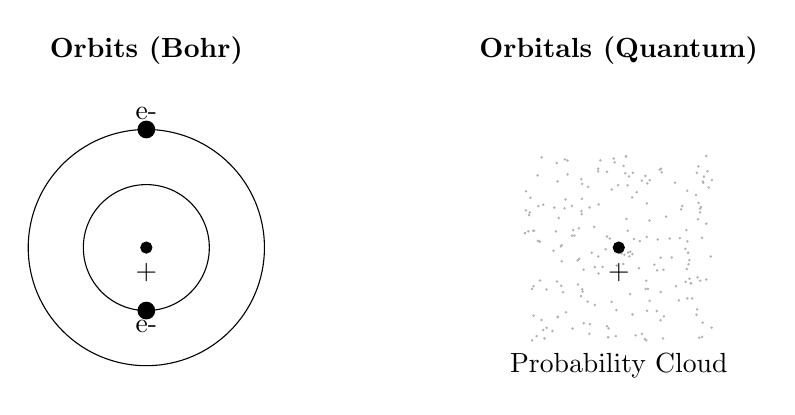
\begin{tikzpicture}
    % Orbits (Bohr Model)
    \node at (-3, 2.5) {\textbf{Orbits (Bohr)}};
    \draw (-3,0) circle (1.5cm);
    \draw (-3,0) circle (0.8cm);
    \filldraw (-3,0) circle (2pt) node[below=2pt] {+};
    \filldraw (-3, 1.5) circle (3pt) node[above] {e-};
    \filldraw (-3, -0.8) circle (3pt) node[below] {e-};

    % Orbitals (Quantum)
    \node at (3, 2.5) {\textbf{Orbitals (Quantum)}};
    % Draw some random dots for electron cloud
    \foreach \i in {1,...,200}
        \fill[black!30] (3+rand*1.2, rand*1.2) circle (0.5pt);
    \filldraw (3,0) circle (2pt) node[below=2pt] {+};
    \node at (3, -1.5) {Probability Cloud};
\end{tikzpicture}
\captionof{figure}{Bohr Orbits vs Quantum Orbitals}
\end{center}

\begin{mnemonicbox}
\mnemonic{"Definite Shape Energy Location" (DSEL)}
\end{mnemonicbox}
\end{solutionbox}

\questionmarks{2(B)(2)}{4}{Classify fuels on the basis of its sources and physical states with one example of each.}

\begin{solutionbox}
\textbf{Answer}:

\begin{center}
\captionof{table}{Classification of Fuels}
\begin{tabulary}{\linewidth}{L L L L}
    \toprule
    \textbf{Classification} & \textbf{Type} & \textbf{Example} & \textbf{Description} \\
    \midrule
    \textbf{Source-based} & Natural & Coal & Formed naturally \\
     & Artificial & Petrol & Man-made \\
    \midrule
    \textbf{Physical state} & Solid & Wood & Solid at room temp \\
     & Liquid & Diesel & Liquid at room temp \\
     & Gaseous & LPG & Gas at room temp \\
    \bottomrule
\end{tabulary}
\end{center}

\begin{mnemonicbox}
\mnemonic{"Natural Artificial, Solid Liquid Gas" (NASLG)}
\end{mnemonicbox}
\end{solutionbox}

\questionmarks{2(B)(3)}{4}{Explain bio-diesel with four important points.}

\begin{solutionbox}
\textbf{Answer}:

\begin{itemize}
    \item \keyword{Source}: Made from vegetable oils, animal fats, or waste cooking oil
    \item \keyword{Process}: Produced by transesterification reaction with methanol/ethanol
    \item \keyword{Properties}: Biodegradable, non-toxic, renewable fuel source
    \item \keyword{Applications}: Used in diesel engines, reduces emissions by 75\%
\end{itemize}

\textbf{Chemical Reaction:}
\begin{center}
    Vegetable Oil + Methanol $\rightarrow$ Bio-diesel + Glycerol
\end{center}

\begin{mnemonicbox}
\mnemonic{"Source Process Properties Applications" (SPPA)}
\end{mnemonicbox}
\end{solutionbox}

\questionmarks{3(A)(1)}{3}{Explain solute, solvent and solution with the help of example.}

\begin{solutionbox}
\textbf{Answer}:

\begin{center}
\captionof{table}{Solute, Solvent, Solution}
\begin{tabulary}{\linewidth}{L L L}
    \toprule
    \textbf{Component} & \textbf{Definition} & \textbf{Example} \\
    \midrule
    \textbf{Solute} & Substance being dissolved & Salt (NaCl) \\
    \textbf{Solvent} & Substance doing the dissolving & Water (H\textsubscript{2}O) \\
    \textbf{Solution} & Homogeneous mixture & Salt water \\
    \bottomrule
\end{tabulary}
\end{center}

\textbf{Example}: Sugar + Water = Sugar solution
\begin{itemize}
    \item Sugar = Solute, Water = Solvent, Sugar water = Solution
\end{itemize}

\begin{mnemonicbox}
\mnemonic{"Solute Solvent Solution" (SSS)}
\end{mnemonicbox}
\end{solutionbox}

\questionmarks{3(A)(2)}{3}{Explain the formation of Electrovalent bond in NaCl.}

\begin{solutionbox}
\textbf{Answer}:

\textbf{Process}:
\begin{itemize}
    \item \keyword{Step 1}: Na loses 1 electron $\rightarrow$ Na\textsuperscript{+} (cation)
    \item \keyword{Step 2}: Cl gains 1 electron $\rightarrow$ Cl\textsuperscript{-} (anion)
    \item \keyword{Step 3}: Electrostatic attraction between Na\textsuperscript{+} and Cl\textsuperscript{-}
\end{itemize}

\textbf{Diagram:}

\begin{center}
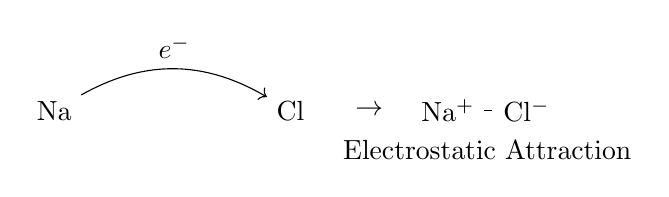
\begin{tikzpicture}
    \node (Na) at (0,0) {Na};
    \node (Cl) at (3,0) {Cl};
    \draw[->, bend left] (Na) to node[midway, above] {$e^-$} (Cl);
    
    \node (NaIon) at (5,0) {Na$^+$};
    \node (ClIon) at (6,0) {Cl$^-$};
    \node at (4,0) {$\rightarrow$};
    
    \draw[dashed] (NaIon) -- (ClIon);
    \node at (5.5, -0.5) {Electrostatic Attraction};
\end{tikzpicture}
\captionof{figure}{NaCl Bond Formation}
\end{center}

\begin{mnemonicbox}
\mnemonic{"Sodium Loses, Chlorine Gains, Attraction Forms" (SLCGAF)}
\end{mnemonicbox}
\end{solutionbox}

\questionmarks{3(A)(3)}{3}{Explain Octane number for gasoline.}

\begin{solutionbox}
\textbf{Answer}:

\begin{center}
\captionof{table}{Octane Number}
\begin{tabulary}{\linewidth}{L L}
    \toprule
    \textbf{Aspect} & \textbf{Description} \\
    \midrule
    \textbf{Definition} & Measure of fuel's resistance to knocking \\
    \textbf{Scale} & 0-100, higher = better anti-knock properties \\
    \textbf{Standard} & n-heptane = 0, iso-octane = 100 \\
    \bottomrule
\end{tabulary}
\end{center}

\textbf{Applications}: High octane fuel prevents engine knocking, improves performance

\begin{mnemonicbox}
\mnemonic{"Octane Opposes Knocking" (OOK)}
\end{mnemonicbox}
\end{solutionbox}

\questionmarks{3(B)(1)}{4}{Explain electrorefining of impure Cu with chemical equations and a labeled diagram.}

\begin{solutionbox}
\textbf{Answer}:

\textbf{Process}:
\begin{itemize}
    \item \keyword{Anode}: Impure copper dissolves
    \item \keyword{Cathode}: Pure copper deposits
    \item \keyword{Electrolyte}: CuSO\textsubscript{4} solution
\end{itemize}

\textbf{Chemical Equations}:
\begin{itemize}
    \item At Anode: Cu $\rightarrow$ Cu\textsuperscript{2+} + 2e\textsuperscript{-}
    \item At Cathode: Cu\textsuperscript{2+} + 2e\textsuperscript{-} $\rightarrow$ Cu
\end{itemize}

\textbf{Diagram:}

\begin{center}
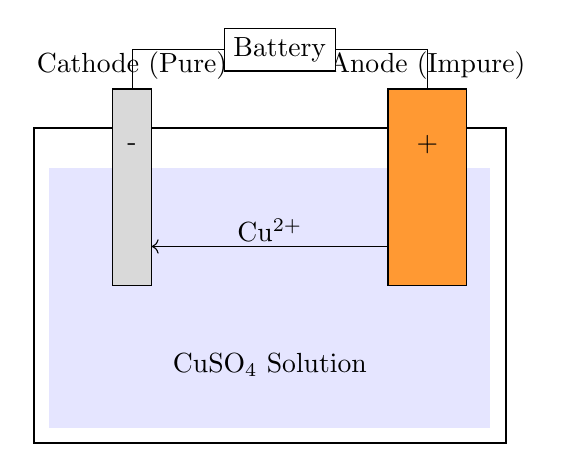
\begin{tikzpicture}
    % Container
    \draw[thick] (0,0) rectangle (6,4);
    \fill[blue!10] (0.2,0.2) rectangle (5.8,3.5);
    \node at (3,1) {CuSO$_4$ Solution};
    
    % Electrodes
    \draw[fill=gray!30] (1,2) rectangle (1.5,4.5); % Cathode
    \node[above] at (1.25,4.5) {Cathode (Pure)};
    \node at (1.25, 3.8) {-};
    
    \draw[fill=orange!80] (4.5,2) rectangle (5.5,4.5); % Anode (Thick)
    \node[above] at (5,4.5) {Anode (Impure)};
    \node at (5, 3.8) {+};
    
    % Circuit
    \draw (1.25,4.5) -- (1.25,5) -- (5,5) -- (5,4.5);
    \node[draw, rectangle, fill=white] at (3.125, 5) {Battery};
    
    % Ions
    \draw[->] (4.5, 2.5) -- (1.5, 2.5);
    \node at (3, 2.7) {Cu$^{2+}$};
\end{tikzpicture}
\captionof{figure}{Electrorefining of Copper}
\end{center}

\begin{mnemonicbox}
\mnemonic{"Anode Dissolves, Cathode Deposits" (ADCD)}
\end{mnemonicbox}
\end{solutionbox}

\questionmarks{3(B)(2)}{4}{Explain preparation of ethene with chemical equation. Also write its two properties and two uses.}

\begin{solutionbox}
\textbf{Answer}:

\textbf{Preparation}:
\begin{center}
    C\textsubscript{2}H\textsubscript{5}OH $\xrightarrow{\Delta}$ C\textsubscript{2}H\textsubscript{4} + H\textsubscript{2}O (Dehydration of ethanol)
\end{center}

\textbf{Properties}:
\begin{itemize}
    \item \keyword{Physical}: Colorless gas, sweet smell
    \item \keyword{Chemical}: Unsaturated, undergoes addition reactions
\end{itemize}

\textbf{Uses}:
\begin{itemize}
    \item \keyword{Industrial}: Manufacturing polyethylene
    \item \keyword{Agricultural}: Plant hormone for fruit ripening
\end{itemize}

\begin{mnemonicbox}
\mnemonic{"Preparation Properties Uses" (PPU)}
\end{mnemonicbox}
\end{solutionbox}

\questionmarks{3(B)(3)}{4}{Explain preparation of Buna-S rubber with chemical equation. Also write its two properties and two uses.}

\begin{solutionbox}
\textbf{Answer}:

\textbf{Preparation}:
Butadiene + Styrene $\rightarrow$ Buna-S rubber (Copolymerization)

\textbf{Chemical Equation}:
\begin{center}
    nC\textsubscript{4}H\textsubscript{6} + nC\textsubscript{8}H\textsubscript{8} $\rightarrow$ [-C\textsubscript{4}H\textsubscript{6}-C\textsubscript{8}H\textsubscript{8}-]\textsubscript{n}
\end{center}

\textbf{Properties}:
\begin{itemize}
    \item \keyword{Mechanical}: Good abrasion resistance
    \item \keyword{Chemical}: Oil and fuel resistant
\end{itemize}

\textbf{Uses}:
\begin{itemize}
    \item \keyword{Automotive}: Tire manufacturing
    \item \keyword{Industrial}: Conveyor belts, hoses
\end{itemize}

\begin{mnemonicbox}
\mnemonic{"Butadiene Styrene Makes Strong Rubber" (BSMSR)}
\end{mnemonicbox}
\end{solutionbox}

\questionmarks{4(A)(1)}{3}{Explain metal clading for the prevention of corrosion of metals.}

\begin{solutionbox}
\textbf{Answer}:

\begin{center}
\captionof{table}{Metal Cladding}
\begin{tabulary}{\linewidth}{L L}
    \toprule
    \textbf{Aspect} & \textbf{Description} \\
    \midrule
    \textbf{Process} & Coating base metal with corrosion-resistant metal \\
    \textbf{Methods} & Hot dipping, electroplating, roll bonding \\
    \textbf{Examples} & Galvanized iron (Zn on Fe), Tin plating \\
    \bottomrule
\end{tabulary}
\end{center}

\textbf{Mechanism}: Protective layer prevents oxygen/moisture contact with base metal

\begin{mnemonicbox}
\mnemonic{"Coating Protects Metal" (CPM)}
\end{mnemonicbox}
\end{solutionbox}

\questionmarks{4(A)(2)}{3}{Explain waterline corrosion with chemical equations and labeled diagram.}

\begin{solutionbox}
\textbf{Answer}:

\textbf{Process}: Differential aeration causes corrosion at water-air interface

\textbf{Chemical Equations}:
\begin{itemize}
    \item Anode: Fe $\rightarrow$ Fe\textsuperscript{2+} + 2e\textsuperscript{-}
    \item Cathode: O\textsubscript{2} + 4H\textsuperscript{+} + 4e\textsuperscript{-} $\rightarrow$ 2H\textsubscript{2}O
\end{itemize}

\textbf{Diagram:}

\begin{center}
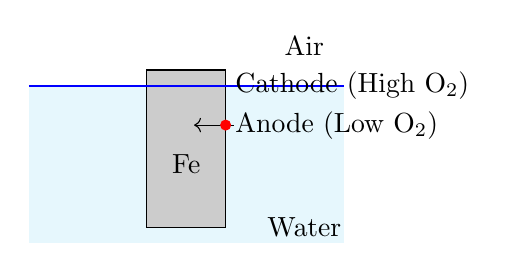
\begin{tikzpicture}
    % Water and Air regions
    \fill[cyan!10] (-2, -2) rectangle (2, 0); % Water
    \node at (1.5, -1.8) {Water};
    \node at (1.5, 0.5) {Air};
    
    % Metal rod
    \fill[gray!40] (-0.5, -1.8) rectangle (0.5, 0.2);
    \draw (-0.5, -1.8) rectangle (0.5, 0.2);
    \node at (0, -1) {Fe};

    % Waterline
    \draw[blue, thick] (-2, 0) -- (2, 0);
    
    % Corrosion spots
    \node[right] at (0.5, 0) {Cathode (High O$_2$)};
    \node[right] at (0.5, -0.5) {Anode (Low O$_2$)};
    
    \draw[->] (0.6, -0.5) -- (0.1, -0.5);
    \fill[red] (0.5, -0.5) circle (2pt); % Corrosion
\end{tikzpicture}
\captionof{figure}{Waterline Corrosion}
\end{center}

\begin{mnemonicbox}
\mnemonic{"Water Air Interface Corrodes" (WAIC)}
\end{mnemonicbox}
\end{solutionbox}

\questionmarks{4(A)(3)}{3}{Explain the working principle of solar cells.}

\begin{solutionbox}
\textbf{Answer}:

\begin{center}
\captionof{table}{Solar Cell Principle}
\begin{tabulary}{\linewidth}{L L}
    \toprule
    \textbf{Component} & \textbf{Function} \\
    \midrule
    \textbf{Photovoltaic effect} & Light energy converts to electrical energy \\
    \textbf{p-n junction} & Creates electric field for charge separation \\
    \textbf{Electron-hole pairs} & Generated when photons hit semiconductor \\
    \bottomrule
\end{tabulary}
\end{center}

\textbf{Process}: Light $\rightarrow$ Electron excitation $\rightarrow$ Current flow $\rightarrow$ Electrical energy

\begin{mnemonicbox}
\mnemonic{"Photo Voltaic Junction Creates Current" (PVJCC)}
\end{mnemonicbox}
\end{solutionbox}

\questionmarks{4(B)(1)}{4}{Demonstrate the function of boundary lubrication with diagram.}

\begin{solutionbox}
\textbf{Answer}:

\textbf{Function}: Thin molecular layer adheres to metal surfaces, prevents direct contact

\textbf{Mechanism}:
\begin{itemize}
    \item \keyword{Formation}: Lubricant molecules orient on metal surface
    \item \keyword{Protection}: Reduces friction and wear between surfaces
    \item \keyword{Load bearing}: Supports load when fluid film breaks down
\end{itemize}

\textbf{Diagram:}

\begin{center}
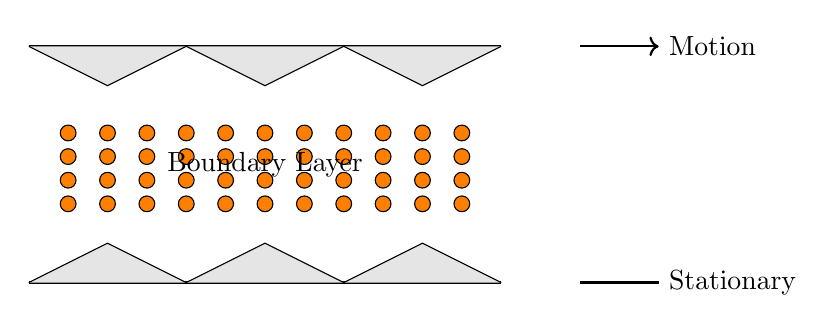
\begin{tikzpicture}
    % Surfaces
    \draw[thick] (0,3) -- (6,3); % Top surface
    \draw[thick] (0,0) -- (6,0); % Bottom surface
    
    % Aspirities
    \draw[fill=gray!20] (0,3) -- (1,2.5) -- (2,3) -- (3,2.5) -- (4,3) -- (5,2.5) -- (6,3);
    \draw[fill=gray!20] (0,0) -- (1,0.5) -- (2,0) -- (3,0.5) -- (4,0) -- (5,0.5) -- (6,0);
    
    % Lubricant Molecules (Circles)
    \foreach \x in {0.5, 1, ..., 5.5} {
        \draw[fill=orange] (\x, 1) circle (0.1);
        \draw[fill=orange] (\x, 1.3) circle (0.1);
        \draw[fill=orange] (\x, 1.6) circle (0.1);
        \draw[fill=orange] (\x, 1.9) circle (0.1);
    }
    \node at (3, 1.5) {Boundary Layer};
    
    % Motion arrows
    \draw[->, thick] (7, 3) -- (8, 3) node[right] {Motion};
    \draw[thick] (7, 0) -- (8, 0) node[right] {Stationary};
\end{tikzpicture}
\captionof{figure}{Boundary Lubrication}
\end{center}

\begin{mnemonicbox}
\mnemonic{"Boundary Barriers Prevent Metal Contact" (BBPMC)}
\end{mnemonicbox}
\end{solutionbox}

\questionmarks{4(B)(2)}{4}{Explain how viscosity is measured through redwood viscometer with labelled diagram.}

\begin{solutionbox}
\textbf{Answer}:

\textbf{Principle}: Time taken for fixed volume of oil to flow through standard orifice

\textbf{Procedure}:
\begin{itemize}
    \item \keyword{Setup}: Fill oil chamber, heat to required temperature
    \item \keyword{Measurement}: Record time for 50ml oil flow
    \item \keyword{Calculation}: Viscosity = Time $\times$ Constant
\end{itemize}

\textbf{Diagram:}

\begin{center}
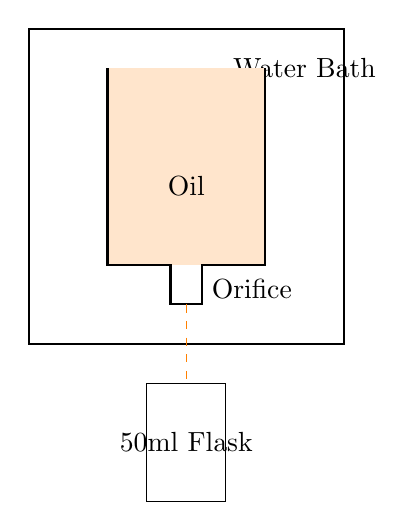
\begin{tikzpicture}
    % Water Bath
    \draw[thick] (0,0) rectangle (4,4);
    \node at (3.5, 3.5) {Water Bath};
    
    % Oil Cup
    \fill[orange!20] (1,1) rectangle (3,3.5);
    \draw[thick] (1,3.5) -- (1,1) -- (1.8,1) -- (1.8,0.5) -- (2.2,0.5) -- (2.2,1) -- (3,1) -- (3,3.5);
    \node at (2,2) {Oil};
    
    % Orifice
    \draw[thick] (1.9, 0.5) -- (2.1, 0.5);
    \node[right] at (2.2, 0.7) {Orifice};
    
    % Flask
    \draw (1.5, -2) -- (1.5, -0.5) -- (2.5, -0.5) -- (2.5, -2) -- cycle;
    \node at (2, -1.25) {50ml Flask};
    
    % Stream
    \draw[dashed, orange] (2, 0.5) -- (2, -0.5);
\end{tikzpicture}
\captionof{figure}{Redwood Viscometer}
\end{center}

\begin{mnemonicbox}
\mnemonic{"Redwood Records Time" (RRT)}
\end{mnemonicbox}
\end{solutionbox}

\questionmarks{4(B)(3)}{4}{Define: Semiconductor, Insulating material, Elastomer, Addition polymerization.}

\begin{solutionbox}
\textbf{Answer}:

\begin{center}
\captionof{table}{Definitions}
\begin{tabulary}{\linewidth}{L L}
    \toprule
    \textbf{Term} & \textbf{Definition} \\
    \midrule
    \textbf{Semiconductor} & Material with electrical conductivity between conductor and insulator \\
    \textbf{Insulating material} & Material that resists flow of electric current \\
    \textbf{Elastomer} & Polymer with elastic properties, can stretch and return to original shape \\
    \textbf{Addition polymerization} & Monomers join without elimination of small molecules \\
    \bottomrule
\end{tabulary}
\end{center}

\textbf{Examples}: Si (semiconductor), Rubber (insulator), Rubber (elastomer), Polyethylene (addition)

\begin{mnemonicbox}
\mnemonic{"Semi Insulating Elastic Addition" (SIEA)}
\end{mnemonicbox}
\end{solutionbox}

\questionmarks{5(A)(1)}{3}{Solve: Calculate the pH and pOH of 0.004 M HCl aqueous solution. (log 4 = 0.6021)}

\begin{solutionbox}
\textbf{Answer}:

\textbf{Given}: [HCl] = 0.004 M = 4 $\times$ 10\textsuperscript{-3} M

\textbf{Solution}:
\begin{itemize}
    \item HCl is strong acid, completely ionizes
    \item [H\textsuperscript{+}] = [HCl] = 4 $\times$ 10\textsuperscript{-3} M
    \item pH = -log[H\textsuperscript{+}] = -log(4 $\times$ 10\textsuperscript{-3})
    \item pH = -log 4 - log 10\textsuperscript{-3} = -0.6021 + 3 = 2.398
    \item pOH = 14 - pH = 14 - 2.398 = 11.602
\end{itemize}

\textbf{Answer}: pH = 2.40, pOH = 11.60

\begin{mnemonicbox}
\mnemonic{"Strong Acid, Simple Calculation" (SASC)}
\end{mnemonicbox}
\end{solutionbox}

\questionmarks{5(A)(2)}{3}{Describe extrinsic semiconductors and it types with examples.}

\begin{solutionbox}
\textbf{Answer}:

\begin{center}
\captionof{table}{Extrinsic Semiconductors}
\begin{tabulary}{\linewidth}{L L L L}
    \toprule
    \textbf{Type} & \textbf{Dopant} & \textbf{Majority Carriers} & \textbf{Example} \\
    \midrule
    \textbf{n-type} & Donor atoms (Group V) & Electrons & Si + P \\
    \textbf{p-type} & Acceptor atoms (Group III) & Holes & Si + B \\
    \bottomrule
\end{tabulary}
\end{center}

\textbf{Properties}:
\begin{itemize}
    \item \keyword{n-type}: Extra electrons increase conductivity
    \item \keyword{p-type}: Electron deficiency creates positive holes
\end{itemize}

\begin{mnemonicbox}
\mnemonic{"n-negative electrons, p-positive holes" (nnep)}
\end{mnemonicbox}
\end{solutionbox}

\questionmarks{5(A)(3)}{3}{Distinguish between thermoplastic polymers and thermosetting polymer (Four points of each)}

\begin{solutionbox}
\textbf{Answer}:

\begin{center}
\captionof{table}{Thermoplastic vs Thermosetting}
\begin{tabulary}{\linewidth}{L L L}
    \toprule
    \textbf{Property} & \textbf{Thermoplastic} & \textbf{Thermosetting} \\
    \midrule
    \textbf{Structure} & Linear/branched chains & Cross-linked network \\
    \textbf{Heat effect} & Softens on heating & Does not soften \\
    \textbf{Reversibility} & Reversible process & Irreversible process \\
    \textbf{Examples} & PVC, PE, PS & Bakelite, Epoxy \\
    \bottomrule
\end{tabulary}
\end{center}

\begin{mnemonicbox}
\mnemonic{"Thermo-plastic = Reversible, Thermo-setting = Permanent" (TPRTSP)}
\end{mnemonicbox}
\end{solutionbox}

\questionmarks{5(B)(1)}{4}{Describe hydrogen bond and its types with examples.}

\begin{solutionbox}
\textbf{Answer}:

\textbf{Definition}: Weak electrostatic attraction between hydrogen and electronegative atoms

\textbf{Types}:
\begin{center}
\captionof{table}{Hydrogen Bond Types}
\begin{tabulary}{\linewidth}{L L L}
    \toprule
    \textbf{Type} & \textbf{Description} & \textbf{Example} \\
    \midrule
    \textbf{Intermolecular} & Between different molecules & H\textsubscript{2}O$\cdot\cdot\cdot$H\textsubscript{2}O \\
    \textbf{Intramolecular} & Within same molecule & o-nitrophenol \\
    \bottomrule
\end{tabulary}
\end{center}

\textbf{Characteristics}:
\begin{itemize}
    \item \keyword{Strength}: 5-40 kJ/mol
    \item \keyword{Requirements}: H bonded to F, O, N
\end{itemize}

\textbf{Diagram:}

\begin{center}
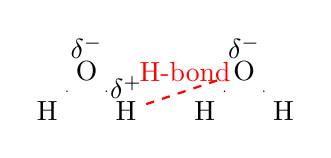
\begin{tikzpicture}
    \node (O1) at (0,0) {O};
    \node (H1a) at (-0.5,-0.5) {H};
    \node (H1b) at (0.5,-0.5) {H};
    \draw (O1) -- (H1a);
    \draw (O1) -- (H1b);
    \node [above=1pt] at (H1b) {$\delta^+$};
    \node [above=1pt] at (O1) {$\delta^-$};
    
    \node (O2) at (2,0) {O};
    \node (H2a) at (1.5,-0.5) {H};
    \node (H2b) at (2.5,-0.5) {H};
    \draw (O2) -- (H2a);
    \draw (O2) -- (H2b);
    \node [above=1pt] at (O2) {$\delta^-$};
    
    \draw[dashed, red, thick] (H1b) -- (O2);
    \node[red, above] at (1.25, -0.25) {H-bond};
\end{tikzpicture}
\captionof{figure}{Hydrogen Bonding in Water}
\end{center}

\begin{mnemonicbox}
\mnemonic{"Hydrogen Needs FON friends" (Fluorine, Oxygen, Nitrogen)}
\end{mnemonicbox}
\end{solutionbox}

\questionmarks{5(B)(2)}{4}{Differentiate between Primary cell and Secondary cell. (Four points)}

\begin{solutionbox}
\textbf{Answer}:

\begin{center}
\captionof{table}{Primary vs Secondary Cell}
\begin{tabulary}{\linewidth}{L L L}
    \toprule
    \textbf{Aspect} & \textbf{Primary Cell} & \textbf{Secondary Cell} \\
    \midrule
    \textbf{Rechargeability} & Non-rechargeable & Rechargeable \\
    \textbf{Reaction} & Irreversible & Reversible \\
    \textbf{Cost} & Low initial cost & High initial cost \\
    \textbf{Examples} & Dry cell, alkaline & Lead-acid, Li-ion \\
    \bottomrule
\end{tabulary}
\end{center}

\textbf{Applications}:
\begin{itemize}
    \item \keyword{Primary}: Remote controls, flashlights
    \item \keyword{Secondary}: Cars, phones, laptops
\end{itemize}

\begin{mnemonicbox}
\mnemonic{"Primary = Permanent, Secondary = Reversible" (PPSR)}
\end{mnemonicbox}
\end{solutionbox}

\questionmarks{5(B)(3)}{4}{Describe construction, working and chemical equations of lead-acid storage cell with a labelled diagram.}

\begin{solutionbox}
\textbf{Answer}:

\textbf{Construction}:
\begin{itemize}
    \item \keyword{Anode}: Lead (Pb)
    \item \keyword{Cathode}: Lead dioxide (PbO\textsubscript{2})
    \item \keyword{Electrolyte}: Dilute H\textsubscript{2}SO\textsubscript{4}
\end{itemize}

\textbf{Chemical Equations}:
\begin{itemize}
    \item \keyword{Discharge}: Pb + PbO\textsubscript{2} + 2H\textsubscript{2}SO\textsubscript{4} $\rightarrow$ 2PbSO\textsubscript{4} + 2H\textsubscript{2}O
    \item \keyword{Charge}: 2PbSO\textsubscript{4} + 2H\textsubscript{2}O $\rightarrow$ Pb + PbO\textsubscript{2} + 2H\textsubscript{2}SO\textsubscript{4}
\end{itemize}

\textbf{Diagram}:

\begin{center}
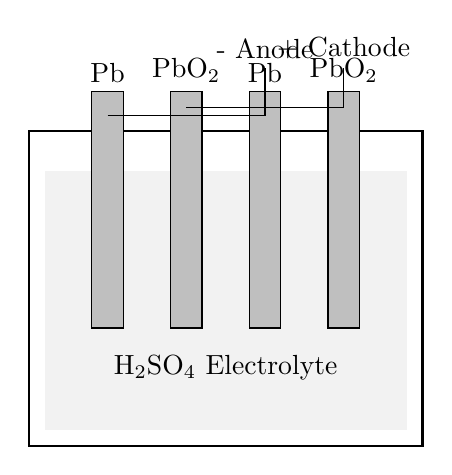
\begin{tikzpicture}
    % Container
    \draw[thick] (0,0) rectangle (5,4);
    \fill[gray!10] (0.2,0.2) rectangle (4.8,3.5);
    \node at (2.5, 1) {H$_2$SO$_4$ Electrolyte};
    
    % Plates
    \foreach \x in {1, 2, 3, 4} {
        \draw[fill=gray!50] (\x-0.2, 1.5) rectangle (\x+0.2, 4.5);
    }
    
    % Terminals
    \node[above] at (1, 4.5) {Pb};
    \node[above] at (2, 4.5) {PbO$_2$};
    \node[above] at (3, 4.5) {Pb};
    \node[above] at (4, 4.5) {PbO$_2$};
    
    % Bus bars
    \draw (1,4.2) -- (3,4.2) -- (3,4.8) node[above] {- Anode};
    \draw (2,4.3) -- (4,4.3) -- (4,4.8) node[above] {+ Cathode};

\end{tikzpicture}
\captionof{figure}{Lead-Acid Battery}
\end{center}

\textbf{Working}: Chemical energy converts to electrical energy during discharge

\begin{mnemonicbox}
\mnemonic{"Lead Acid Storage = Reversible Energy" (LASRE)}
\end{mnemonicbox}
\end{solutionbox}

\end{document}
